%%%%%%%%%%%%%%%%%%%%%%%%%%%%%%%%%%%%%%%%%%%%%%%%%%%%%%%%%%%%%  
%
% Sprawozdanie MOW
% TEMAT PROJEKTU: 
% AUTOR: 	Krzysztof Belewicz
%			Paweł Pieńczuk
% 23.01.2020
%
%%%%%%%%%%%%%%%%%%%%%%%%%%%%%%%%%%%%%%%%%%%%%%%%%%%%%%%%%%%%%

\documentclass[a4paper,11pt,twoside]{mwrep}  %bylo report
\usepackage[utf8]{inputenc} %ISO-8859-2 
\usepackage[UKenglish,polish]{babel} 
\usepackage[T1]{fontenc} 
\usepackage{mathptmx}
\usepackage[scaled=.90]{helvet}
\usepackage{courier}
\usepackage{gensymb} %\degree
%\usepackage[pdftex]{graphicx} 
%\usepackage{pdfpages} 
%\usepackage{wrapfig}
%\usepackage{hyperref} 
%\usepackage{gensymb}
% tablice
%\usepackage{ctable}
%\usepackage{threeparttablex}
%\usepackage{booktabs}
% grafiki
\usepackage{graphicx}
\usepackage{subfig}
\usepackage{float}
%% matematyka i greckie literki w jednostkach
\usepackage{amsmath}
\usepackage{textgreek}
%% wstawki pdf
%\usepackage{pdfpages}
% wstawki z kodem 
\usepackage{listings}
\usepackage{color}
\usepackage{url}
% Linki
\makeatletter
\g@addto@macro{\UrlBreaks}{\UrlOrds}
\expandafter\def\expandafter\UrlBreaks\expandafter{\UrlBreaks%  save the current one
  \do\a\do\b\do\c\do\d\do\e\do\f\do\g\do\h\do\i\do\j%
  \do\k\do\l\do\m\do\n\do\o\do\p\do\q\do\r\do\s\do\t%
  \do\u\do\v\do\w\do\x\do\y\do\z\do\A\do\B\do\C\do\D%
  \do\E\do\F\do\G\do\H\do\I\do\J\do\K\do\L\do\M\do\N%
  \do\O\do\P\do\Q\do\R\do\S\do\T\do\U\do\V\do\W\do\X%
  \do\Y\do\Z}
  
%\usepackage[paper=A4]{typearea}
%marginesy 
\usepackage[ bindingoffset = 0cm, hmargin = 2cm, vmargin = 2cm]{geometry} 
%interlinia 
\linespread{1} 

\widowpenalty=10000 % ostatni wierszrkapitu nie zostanie przeniesiony na następną stronę 
\clubpenalty=10000 % pierwszy wiersz akapitu nie będzie kończył strony (nie używam tego ustawienia)
\hbadness= 1450 %% zmniejsza liczę wyświetlanych ostrzeżeń (można zwiększyć, ale bez przesady)
\hfuzz = 0pt %% tekst może sterczeć ma marginesie na 1,5pt (ok. 0,5mm)

\clubpenalty=10000 %nie pozostawia sierot
\brokenpenalty=10000 %nie dzieli stron je»eli podziaª wyrazu
\sloppy %zakaz wydªu»ania lini

%wcięcia 
\setlength{\parindent}{1cm} 
\setcounter{secnumdepth}{2} %only sections and subsections are numbered 
\setcounter{tocdepth}{2} %table of contents shows up to three levels 

%\newcommand\tab[1][1cm]{\hspace*{#1}}

\begin{document} 



%%%%%%%%%%%%%%%%%%%%%%%%%%%%%%%%%%%%%%%
%			STRONA TYTUŁOWA
%%%%%%%%%%%%%%%%%%%%%%%%%%%%%%%%%%%%%%%

\begin{titlepage} 
{\begingroup
\centering 

\vspace*{15\baselineskip} 

{\Huge Metody Odkrywania Wiedzy}
\vspace*{1\baselineskip}

{\huge Dokumentacja końcowa projektu}

\vspace*{3\baselineskip}
{\LARGE „Predykcja zużycia energii na podstawie danych czujnikowych”}
\\[\baselineskip]

\vspace*{20\baselineskip} 
{\Large 
Krzysztof Belewicz\\
Paweł Pieńczuk\par} 

\vspace*{1\baselineskip}
\today

\endgroup\clearpage}
\end{titlepage} 

\large %trochę cheat na objętość

\begingroup
\let\clearpage\relax
\chapter{Opis projektu} %Interpretacja tematu

Celem projektu było wyznaczenie całkowitego zużycia energii dla zadanej chwili czasu, tzn. sumy poborów sprzętów AGD (kolumna \textit{Appliances}) i oświetlenia (kolumna \textit{lights}). 
Zbiór danych został pozyskany z archiwum dostępnego na stronie: 
{\url{https://archive.ics.uci.edu/ml/datasets/Appliances+energy+prediction}}. Pojęciem docelowym jest wartość całkowitej pobieranej mocy przez gospodarstwo domowe. W ramach projektu zdecydowano się na oddzielne wykonania zadania regresji dla celu \textit{Appliances} i celu \textit{lights}, ze względu na hipotezę, że modele je wyznaczające mogą mieć inne właściwości.
\par
Dokonano selekcji atrybutów za pomocą trzech algorytmów opisanych w rozdziale \ref{chap:selekcja}. Przeprowadzono procedurę oceny algorytmów liniowej regresji, drzew regresji oraz kawałkami liniowej regresji. 

\endgroup

\begingroup
\let\clearpage\relax
\chapter{Opis danych}

\section{Charakterystyka danych}

Dane wykorzystywane do eksperymentów zostały zebrane za pomocą sieci czujników w niewielkim domu w czasie 4.5 miesiąca. 
Składają się z:
\begin{itemize}
\item[$\bullet$] daty i godziny pomiaru,
\item[$\bullet$] poboru energii sprzętów domowych [$Wh$],
\item[$\bullet$] poboru energii oświetlenia [$Wh$],
\item[$\bullet$] pomiarów temperatury i wilgotności dla 8 różnych pomieszczeń ([\degree $C$], [$\%$]),
\item[$\bullet$] pomiarów temperatury i wilgotności dla zewnętrznej, północnej strony budynku ([\degree $C$], [$\%$]),
\item[$\bullet$] danych z pobliskiej stacji pogodowej:
	\begin{itemize}
	\item[$\circ$] temperatura powietrza [\degree $C$],
	\item[$\circ$] temperatura punktu rosy [\degree $C$],
	\item[$\circ$] ciśnienie atmosferyczne [$mm~Hg$],
	\item[$\circ$] wilgotność [$\%$],
	\item[$\circ$] prędkość wiatru [$m/s$],
	\item[$\circ$] widoczność [$km$].
	\end{itemize}
\end{itemize}

\section{Przygotowanie danych}
Każdy pomiar został uśredniony z 3 próbek wykonanych w równych odstępach co ok. 3,3 min. W ramach przygotowania danych, data i godzina pomiaru zostały rozdzielone na cztery oddzielne kolumny, zawierające miesiąc, dzień, godzinę i minutę pomiaru.
\par
Liczba wszystkich obserwacji, zebranych w pliku \textit{energydata\_complete.csv} wynosi 19735. Celem przyspieszenia obliczeń, algorytmy przedstawione w zadaniu zostały wykonane na danych zawierających 2000 pierwszych rekordów zmienna \textit{testDataLength}. Wszystkie operacje dot. przygotowania danych są wykonane w funkcji \textit{data\_org}.
\endgroup


%\pagebreak
\clearpage

\begingroup
\let\clearpage\relax
\chapter{Selekcja atrybutów}\label{chap:selekcja}

Aby zapobiec nadmiernemu dopasowaniu, stosuje się selekcję atrybutów, która wybiera kilka najważniejszych atrybutów do późniejszego stworzenia modeli. Po zastosowaniu selekcji, modele oparte o ograniczoną liczbę atrybutów zwykle są lepsze od opartych o wszystkie atrybuty. Istnieje wiele metod selekcji atrybutów; w ramach projektu zostało sprawdzone kilka metod (w nawiasach umieszczono opcję type funkcji \textit{feature\_selection}):
\begin{itemize}
	\item[$\bullet$] prosty filtr statystyczny (\textit{,,simple''}) - pomiędzy każdym z atrybutów a celem regresji stosuje się miarę statystyczną, która określa zależność celu od danego atrybutu (dalej ,,miara zależności''). Następnie wybiera się kilka atrybutów o największej ,,mierze zależności''. W ramach regresji pomiędzy atrybutami ciągłymi zastosowano współczynnik korelacji (Pearsona);
	\item[$\bullet$] bazująca na drzewach losowych (\textit{,,rf''}) - w tym celu wykorzystano pakiet randomForest i jego wbudowaną opcję zwracają parametr IMPORTANCE (bazujący na mierze MSE), o możliwości konfiguracji ilości drzew, w badaniu wykorzystano generowanie 500 drzew;
	\item[$\bullet$] metoda RRELIEF (\textit{,,relief''}) - wersja algorytmu RELIEF do zastosowań w zadaniu regresji. Algorytm RELIEF, początkowo zaprojektowany dla zadania klasyfikacji binarnej, polega na losowym wybraniu obserwacji (jednego rekordu klasy+atrybuty). Następnie wyszukuje się \textit{k} najbardziej podobnych obserwacji tej samej klasy, oraz \textit{k} klasy przeciwnej. Dla każdego atrybutu oblicza się wagę istotności. Po wykonaniu \textit{K} operacji, wykonuje się średnią wag istotności. Atrybuty segreguje się według wag istotności. W zadaniu regresji stosuje się inne funkcje obliczające wagę np. funkcję rozkładu. W projekcie \textit{k=3}, \textit{K=50}.
\end{itemize}
	
\par
W ramach projektu stosuje się następujące podejście: dla każdej wymienionej metody wykonuje się selekcję połowy atrybutów (\textit{part=0.5}) atrybutów, następnie wyznaczoną formułę aplikuje się do stworzenia modelu \textit{rpart()}, i procedurze oceny (10-krotnej walidacji krzyżowej \textit{model\_eval()})\footnote{Więcej nt. procedury walidacji krzyżowej w rozdziale \ref{sect:proceduryOceny}}. Następnie największy współczynnik korelacji Pearsona wyznacza najlepszą metodę selekcji atrybutów oraz formułę do stworzenia modelu.

\section{Wyniki selekcji atrybutów}

Na rysunkach \ref{fig:rf_app} -- \ref{fig:relief_app} przedstawiono wyniki każdej z selekcji. Dla \textit{randomForest} i \textit{simple.filter} atrybut \textit{hours} dominuje nad pozostałymi. W tabeli \ref{table:wynikiSelekcji} przedstawiono porównanie wyników każdej z selekcji. Wynika z tego, że atrybuty wyznaczone funkcją \textit{simple.filter} pozwalają na najlepsze wyznaczenie modelu. Dla porównania przedstawiono też wynik walidacji krzyżowej dla modelu opartego o wszystkie atrybuty. Tylko selekcja atrybutów za pomocą \textit{simple.filter} pozwala na poprawę dla obecnych warunków testowych (dostępne dane, ilość selekcjonowanych argumentów, algorytm do walidacji krzyżowej). W związku z wynikami, atrybuty wyznaczono za pomocą prostego filtru statystycznego posłużą w dalszej konstrukcji modelów.

 \begin{figure}[!h]
    \centering 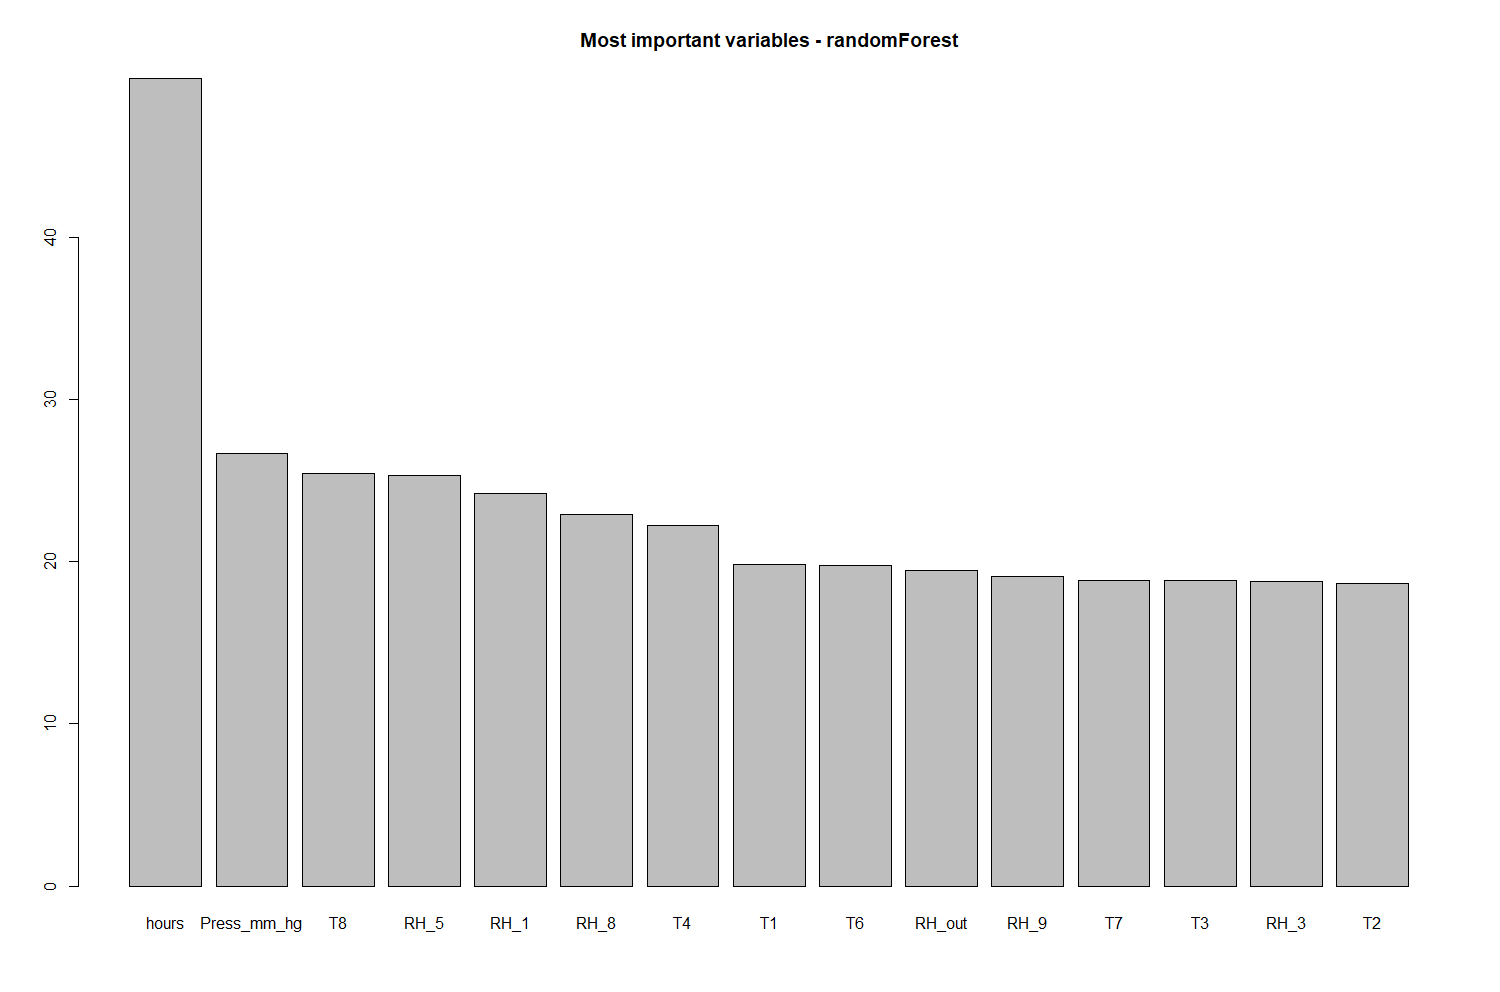
\includegraphics[scale=0.4]{../rf_lights.png}
    \caption{Wyniki selekcji z wykorzystaniem pakietu \textit{randomForest}; cel: lights}
    \label{fig:rf_lights}
\end{figure}

 \begin{figure}[!h]
    \centering 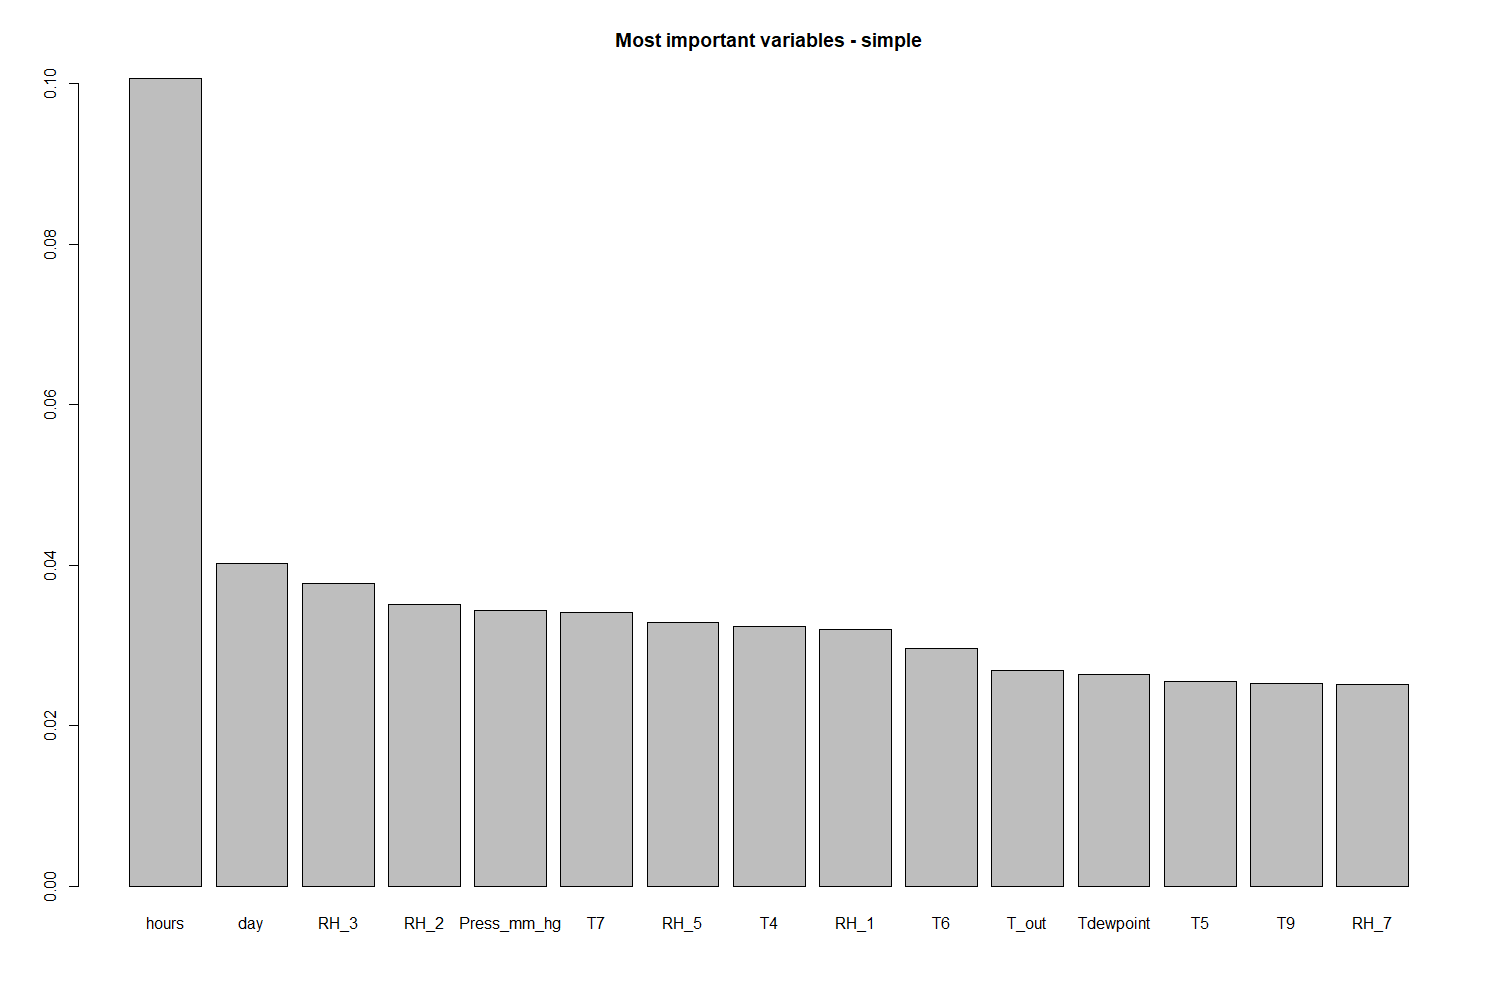
\includegraphics[scale=0.4]{../simple_lights.png}
    \caption{Wyniki selekcji z wykorzystaniem funkcji \textit{simple.filter}; cel: lights}
    \label{fig:simple_lights}
\end{figure}

 \begin{figure}[!h]
    \centering 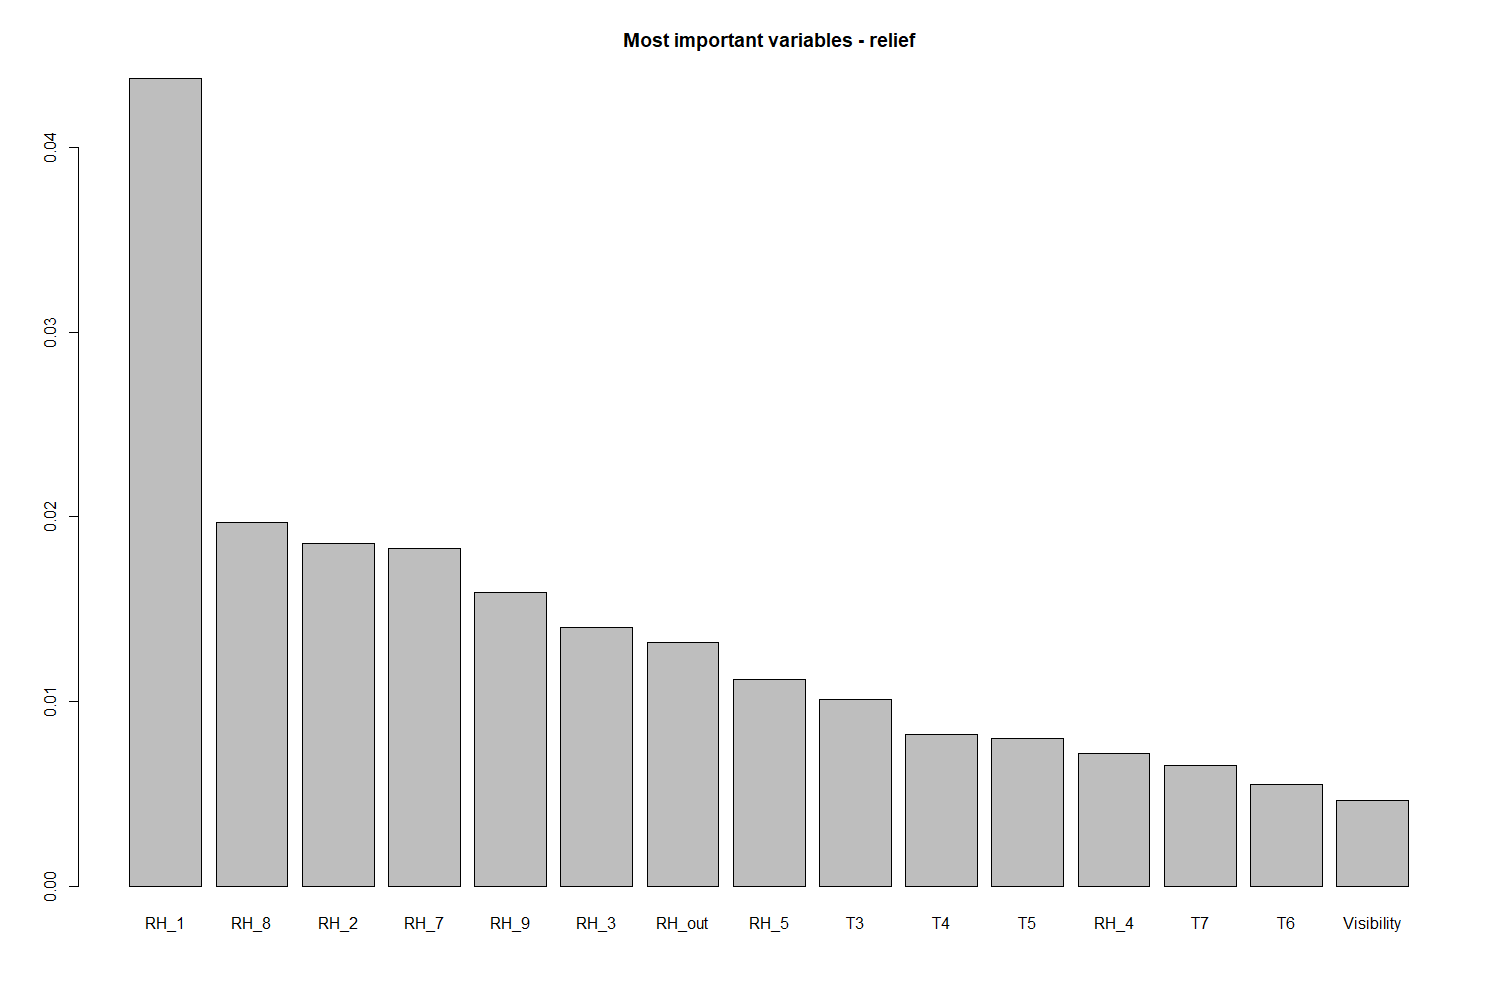
\includegraphics[scale=0.4]{../relief_lights.png}
    \caption{Wyniki selekcji z wykorzystaniem  funkcji \textit{rrelief.filter}; cel: lights}
    \label{fig:relief_lights}
\end{figure}

 \begin{figure}[!h]
    \centering 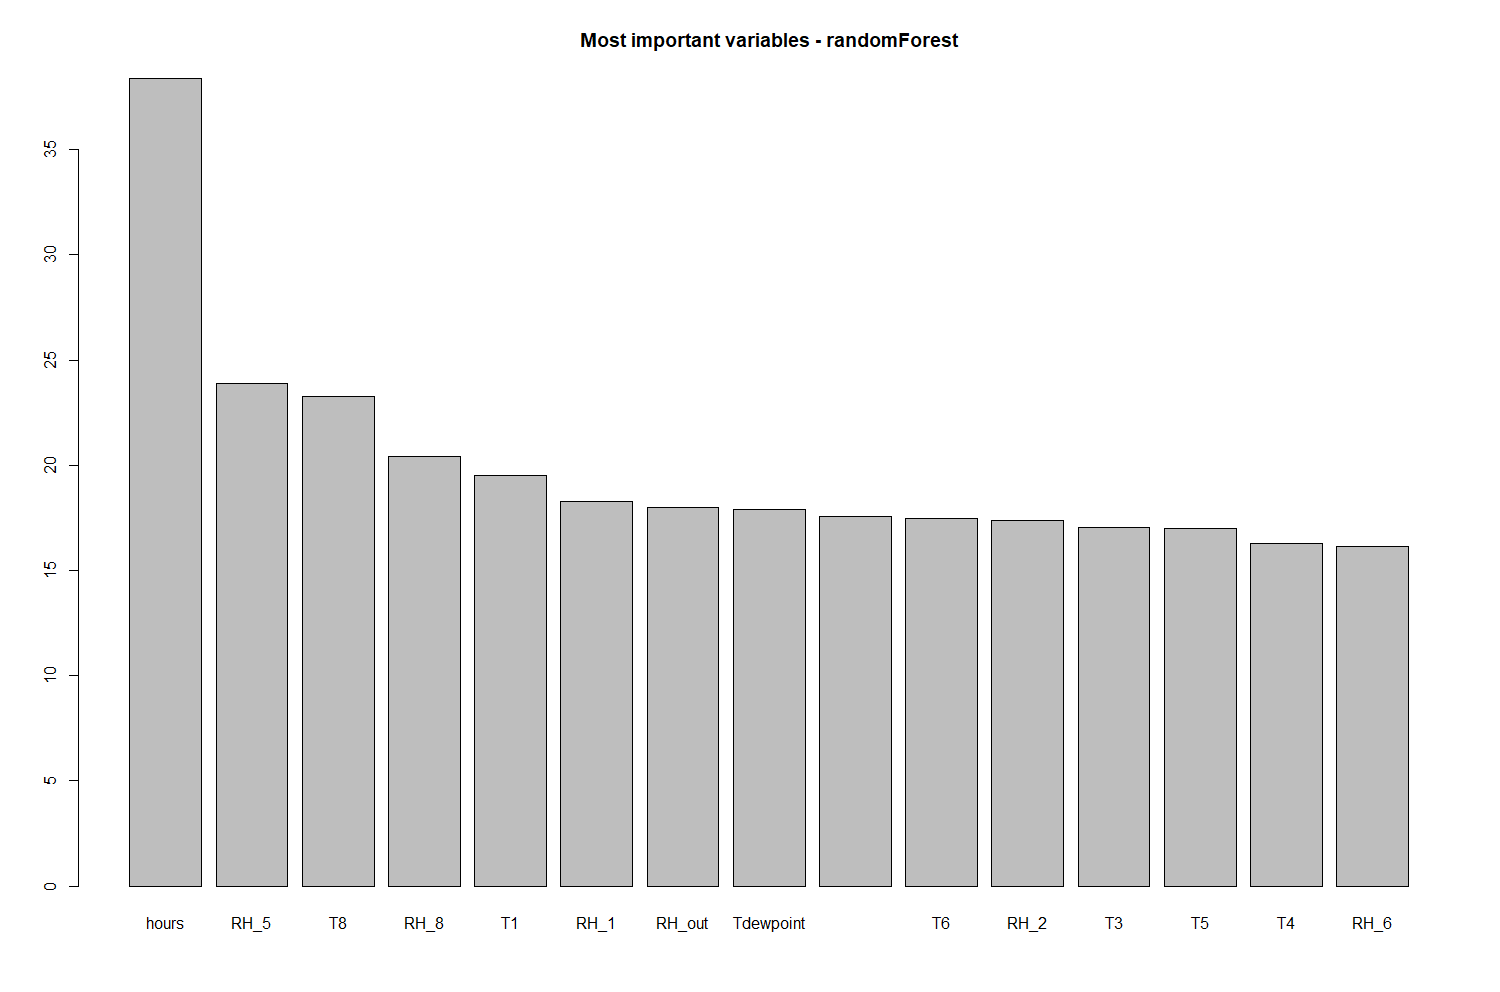
\includegraphics[scale=0.4]{../rf_app.png}
    \caption{Wyniki selekcji z wykorzystaniem pakietu \textit{randomForest}; cel: Appliances}
    \label{fig:rf_app}
\end{figure}

 \begin{figure}[!h]
    \centering 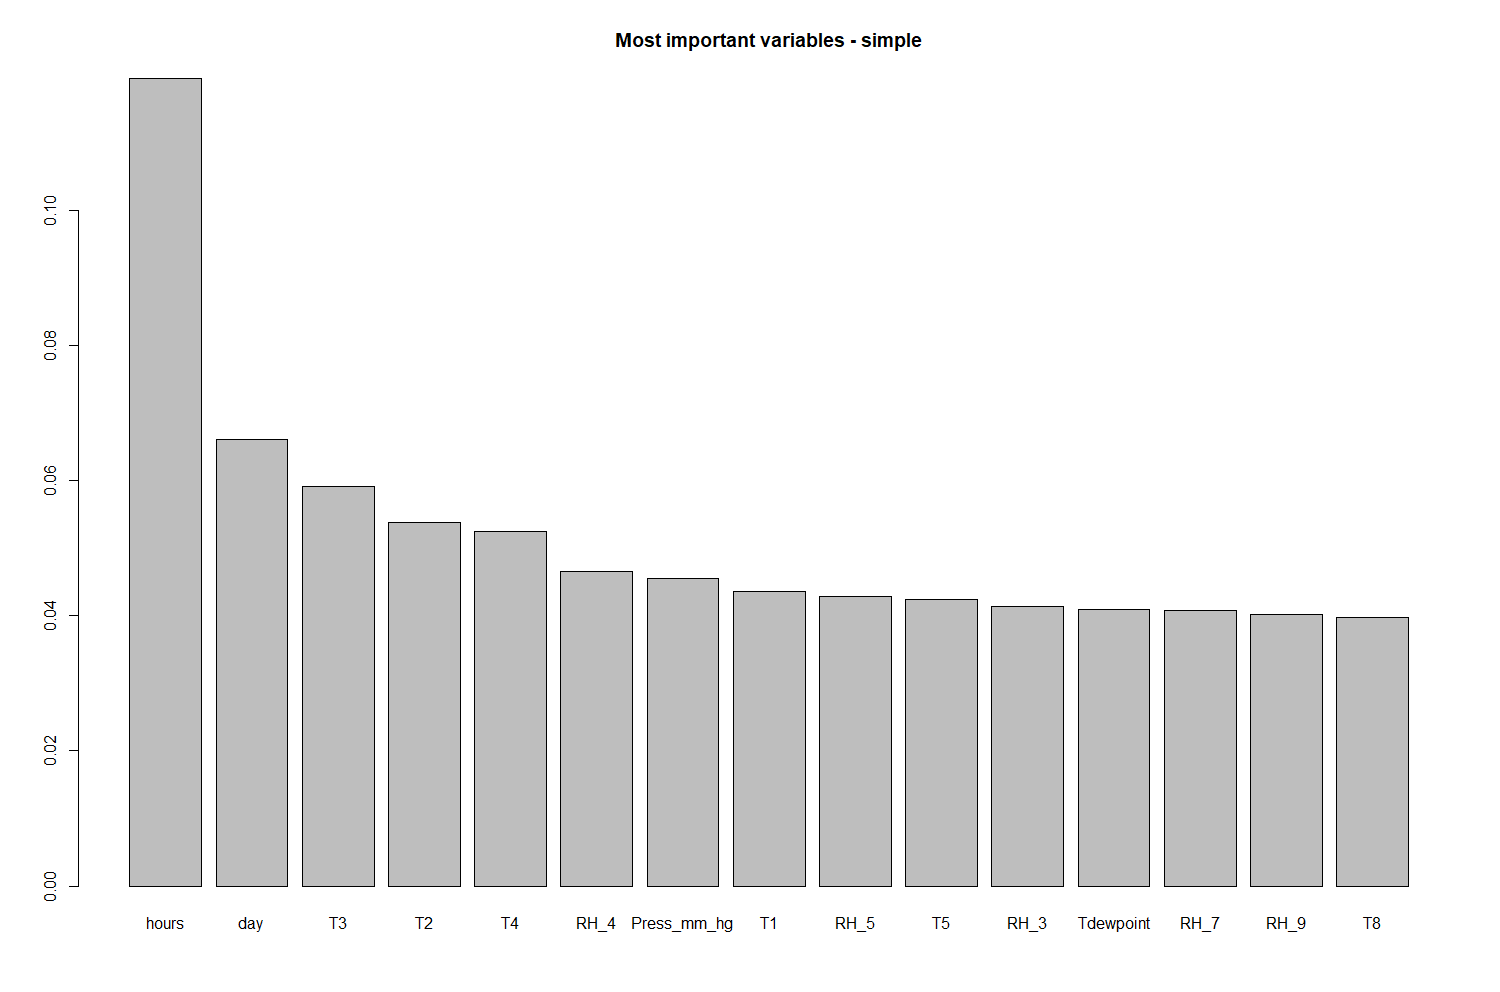
\includegraphics[scale=0.4]{../simple_app.png}
    \caption{Wyniki selekcji z wykorzystaniem funkcji \textit{simple.filter}; cel: Appliances}
    \label{fig:simple_app}
\end{figure}

 \begin{figure}[!h]
    \centering 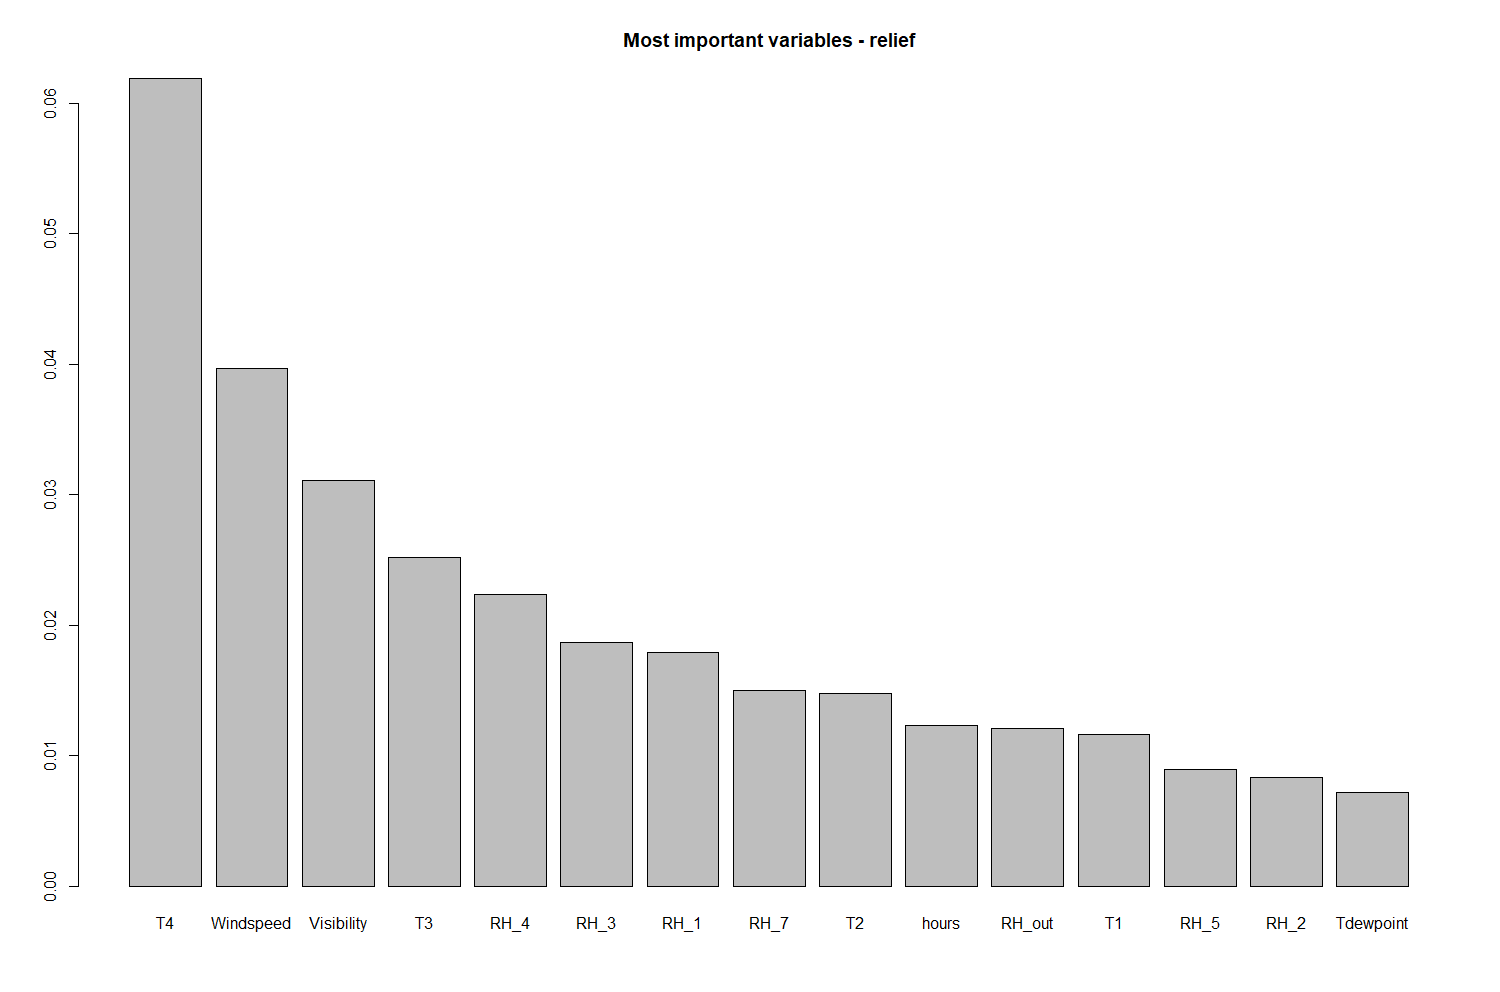
\includegraphics[scale=0.4]{../relief_app.png}
    \caption{Wyniki selekcji z wykorzystaniem  funkcji \textit{rrelief.filter}; cel: Appliances}
    \label{fig:relief_app}
\end{figure}


\begin{table}[!h]  \centering
\caption{Wyniki selekcji atrybutów --- współczynniki korelacji}
\begin{tabular} { c  c  c  c  c } \hline \hline
    \textbf{Parametr} & \textbf{\textit{randomForest}} & \textbf{\textit{simple}} & \textbf{\textit{RELIEF}} & \textbf{bez selekcji}  \\ \hline
    Appliances & 0,555 & 0,616 & 0,553 & 0,585 \\
    lights & 0,672 & 0,759 & 0,691 & 0,757 \\
    \hline \hline
    
\end{tabular}
\label{table:wynikiSelekcji}
\end{table}

\endgroup

\clearpage
\begingroup
\let\clearpage\relax
\chapter{Konstrukcja i ocena modeli}

\section{Metody konstrukcji modeli}
W pierwszym kroku dokonano modelowania za pomocą liniowej regresji. Realizuje ją algorytm \textit{lm()}. Argumentami algorytmu są tylko: formuła (cel+atrybuty) oraz zestaw danych w formie \textit{data.frame}. Algorytm na podstawie średniej lub mediany wyznacza współczynniki funkcji liniowej tj. współczynnik kierunkowy i wyraz wolny. Następnie od każdego atrybuty wyznacza wagę współczynniku kierunkowego oraz jeden wyraz wolny. Zaletą tego algorytmu jest jego prostota i szybkość działania, zaś niewątpliwą wadą jest fakt, że większość procesów zachodzących w świecie nie da się opisać za pomocą liniowych zależności.
\par 
Następnie dokonano modelowania za pomocą drzew regresji (algorytm \textit{rpart()}). Funkcja buduje model rekurencyjnie dzieląc zbiór na mniejsze i wyznaczając dla nich średnią. Dla metody ,,anova'' dedykowanej do zadania regresji kryterium podziału wyznaczone jest na podstawie sum kwadratów dla danego węzła i dla jego potomnych. Algorytm może przyjąć także argumenty na minimalną liczbę podziałów \textit{minsplit} oraz maksymalną głębokość drzewa \textit{maxdepth} (czyli długość pomiędzy korzeniem a liśćmi).
% https://cran.r-project.org/web/packages/rpart/vignettes/longintro.pdf
\par
Pojedyncze modele drzew regresji zazwyczaj cierpią z powodu wysokiej wariancji -- jedną z metod jej redukcji jest tzw. Bagging (\textbf{B}ootstrap \textbf{agg}regat\textbf{ing}). W ramach tej metody tworzona jest pewna liczba zbiorów "bootstrapowych". Dla każdego z tych zbiorów tworzy się nieprzycięte drzewo regresji. Następnie uśrednia się każdy z tych modeli, zmniejszając wariancję i redukując zbytnie dopasowanie. Bagging może zostać zrealizowany za pomocą pakietu \textit{ipred} lub \textit{caret}. Zasada działania modelowania przy pomocy tych pakietów jest podobna, pakiet \textit{caret} pozwala natomiast na łatwą analizę istotności atrybutów. Celem porównania wyników realizowanych przez oba algorytmy, zdecydowano się na użycie ich obu.
\par
Modele oparte o drzewo regresji cierpią z powodu faktu, że w liściach, które reprezentują pewny podzbiór przestrzeni (na której buduje się model), wynikiem jest pojedyncza liczba. Przykładowo dla zależności celu od jednego atrybutu, funkcja reprezentująca model może być nieciągła i stworzona z odcinków o zerowym współczynniku kierunkowym. Dużo lepiej byłoby aproksymować tę zależność funkcją kawałkami liniową.  W tym celu wykorzystuje się regresję kawałkami liniową (\textit{grow.modtree} z pakietu \textit{dmr.regtree}). Za pomocą listy \textit{plr\_args} ograniczono głębokość drzewa do 10 oraz wymuszono co najmniej 2 podziały.
\par
Modele opisane w tym podrozdziale zostały ocenione za pomocą procedury k-krotnej walidacji krzyżowej z wykorzystaniem miar jakości opisanych dalej. 

\vspace*{\fill}
\pagebreak

\section{Miary jakości}\label{sect:ocenamodeli}
Dla zbudowanych modeli oblicza się następujące miary jakości:
\begin{enumerate}
\item
CC - współczynnik korelacji liniowej Pearsona\\
\begin{gather*}
	CC =\frac{cov(P,A)}{var(P) \cdot var(A)}
\end{gather*}
\item
MSE - błąd średniokwadratowy
\begin{gather*}
	MSE = \frac{(p_1-a_1)^2+...+(p_n-a_n)^2}{n}
\end{gather*}
\item
RMSE - pierwiastek z błędu średniokwadratowego
\begin{gather*}
	RMSE = \sqrt{\frac{(p_1-a_1)^2+...+(p_n-a_n)^2}{n}}
\end{gather*}
\item
MAE - średni błąd względny
\begin{gather*}
	MAE = \frac{|p_1-a_1|+...+|p_n-a_n|}{n}
\end{gather*}
\item
RSE - względny błąd kwadratowy
\begin{gather*}
	RSE = \frac{(p_1-a_1)^2+...+(p_n-a_n)^2}{(a_1-\overline{a})^2+...+(a_n-\overline{a})^2}
\end{gather*}
\item
RRSE - pierwiastek ze względnego błędu kwadratowego
\begin{gather*}
	RRSE = \sqrt{\frac{(p_1-a_1)^2+...+(p_n-a_n)^2}{(a_1-\overline{a})^2+...+(a_n-\overline{a})^2}}
\end{gather*}
\item
RAE - błąd względny
\begin{gather*}
	RAE = \frac{|p_1-a_1|+...+|p_n-a_n|}{|a_1-\overline{a}|+...+|a_n-\overline{a}|}
\end{gather*}
\end{enumerate}

\section{Procedury oceny}\label{sect:proceduryOceny}
Aby móc ocenić model pod względem przydatności zastosowano metodę k-krotnej walidacji krzyżowej. Kod zawarto w funkcji \textit{model\_eval()}.
Zbiór testowy jest dzielony losowo na k podzbiorów równej wielkości. W kolejnych iteracjach każdy ze zbiorów jest traktowany jako zbiór testowy, podczas gdy na reszcie danych buduje się model. Następnie modele są uśredniane i następuje predykcja. Po predykcji modelu na zbiorze testowym wyznacza się miary jakości opisane w \ref{sect:ocenamodeli}.      

\pagebreak
\section{Wyniki walidacji krzyżowej}\label{sect:wyniki}
Wyniki 10-krotnej walidacji krzyżowej zostały przedstawione w tabeli \ref{table:wynikiKCV}. Przedstawia ona miary jakości wyznaczone za pomocą tej procedury dla każdego algorytmu. Zauważa się przewagę metod \textit{bootstrapowych} nad innymi. Błędy i współczynniki korelacji dla tych metod osiągają najmniejsze wartości. Ewentualne różnice pomiędzy wynikami algorytmów z pakietów \textit{ipred} i \textit{caret} można tłumaczyć losowością procesu tworzenia ich modelu i/lub procedury oceny. Zauważa się też różnicę pomiędzy predykcją celu \textit{Appliances} a \textit{lights}. Wydaje się to byc zgodne z intuicją --- zwykle światła włącza się w dzień, a wyłącza w nocy. Z kolei różne urządzenia AGD stosuje się w różnych okresach, więc znalezienie szczególnej zależności może być skomplikowanym zadaniem.   

\begin{table}[!h]  \centering
\caption{Walidacja krzyżowa --- porównanie parametrów}
\begin{tabular} { c  c  c  c  c  c  c  c} \hline \hline
    \textbf{Appliances} & \textbf{MSE} & \textbf{RRSE} & \textbf{MAE} & \textbf{RMSE} & \textbf{RAE} & \textbf{CC} & \textbf{RSE} \\ \hline
	\textit{lm()} & 14914.800 & 2.5702027	&  75.20398	& 122.12616	& 1.9553172	& 0.3425775 & 6.6059421 \\
	\textit{rpart()} & 11646.595 &	1.2051757	& 58.13124 & 107.91939 & 1.0320860	& 0.5698647 & 1.4524484 \\
	\textit{ipred} & 9016.412&	1.3234627&	53.02221&	94.95479&	1.0308015&	0.6983742&	1.7515534 \\
	\textit{PLR} & 266453.137	& 0.9929399 &	78.68274&	516.19099&	0.8137909&	0.1532704&	0.9859296 \\
	\textit{caret} & 8958.720& 	1.2985949&	52.82693&	94.65051&	1.0113670&	0.6991588&	1.6863487 \\
    \hline \hline
\textbf{lights} & \textbf{MSE} & \textbf{RRSE} & \textbf{MAE} & \textbf{RMSE} & \textbf{RAE} & \textbf{CC} & \textbf{RSE} \\ \hline
	\textit{lm()} & 63.61679 &	1.6605096 &	5.640188 &	7.976013 &	1.4319283 &	0.50520939 &	2.7572920 \\
	\textit{rpart()} & 38.27473 & 0.8563671 &	3.815467 &	6.186657 &	0.7194938 &	0.74393671 &	0.7333646 \\
	\textit{ipred} & 30.00860 &	0.8274880 &	3.578404 &	5.478011 &	0.7473722 &	0.81096864 &	0.6847364 \\
	\textit{PLR} & 7264.81589 &	0.9960550 &	9.868371 &	85.233889 &	0.7595684 &	0.09086541 &	0.9921255 \\
	\textit{caret} & 30.92202 &	0.8363734 &	3.593142 &	5.560757 &	0.7441449 &	0.80317142 &	0.6995204 \\
    
\end{tabular}
\label{table:wynikiKCV}
\end{table}

\endgroup

%\clearpage
%\pagebreak
\begingroup
\let\clearpage\relax
\chapter{Wnioski}

TODO\\

\endgroup

%%%%%%%%%%%%%%%%%%%%%%%%%%%%%%%%%%%%%%%%%%%%%%%%%%%%%%%%%%%%%

\lstset{language=R, 
		basicstyle=\ttfamily\small,
		frame=lines,
		numbers=left,
		numberstyle=\small\color{blue},
		showtabs=true}

\clearpage		
\pagebreak
Plik: main.r
\lstinputlisting{../R/main.r}
\clearpage

\pagebreak
Plik: data{\_}org.R
\lstinputlisting{../R/data_org.R}
\clearpage

\pagebreak
Plik: feature{\_}selection.R
\lstinputlisting{../R/feature_selection.R}
\clearpage

\pagebreak
Plik: simple.filter.R
\lstinputlisting{../R/simple.filter.R}
\clearpage

\pagebreak
Plik: model{\_}eval.R
\lstinputlisting{../R/model_eval.R}
\clearpage


\end{document}
